
\chapter{Halbleitertechnik}

Im Computer findet man Logikgatter natürlich nicht aus Schaltern, da diese zum einen manuell betätigt werden müssten und zum anderen zu viel Platz brauchen.
Die Logikgatter sollen elektronisch angesteuert werden, sodass zum Beispiel der Schalter umgelegt wird, wenn man Strom anlegt.

In den Anfangszeiten des Computers wurden dafür Relais benutzt.
Diese konnten mit Strom angesteuert werden und agierten dann wie ein Schalter.
Aber auch diese waren bald zu langsam und benötigten sehr viel Platz.

Später verwendete man Radioröhren anstatt Relais.
Schließlich ging man aber zu Halbleiterelementen über und verwendete Transistoren um elektronisch zu schalten.
Bis heute werden diese Transistoren (als Feldeffekttransistoren) im Prozessor verwendet.


\begin{Ziele}
In diesem Kapitel lernst du ...
\begin{itemize}
\item Was Halbleiter sind und was diese mit Leitern und Isolatoren zu tun haben,
\item warum sich die Leitfähigkeit von Halbleitern mit zunehmender Energie ändern lässt,
\item welche typischen Halbleitersensoren in der Technik eingesetzt werden,
\item was eine Halbleiterdiode ist und wozu diese eingesetzt werden kann,
\item wie ein Bipolartransistor aufgebaut ist und welche Anwendungen er besitzt und
\item wie man einen Transistor im Computer zum Schalten verwendet.
\end{itemize}
\end{Ziele}

\section{Grundbegriffe der Halbleitertechnik}

%\begin{code}{1}
\begin{Aufgabe}
Lies dir den nachfolgenden Abschnitt durch und mache dir Notizen in dein Heft!
Insbesondere die folgenden Fragen sollten beantwortet werden:
\begin{enumerate}
\item Was versteht man unter den Begriffen \emph{Valenzelektronen}, \emph{Valenzband}, \emph{Leitungsband} und \emph{freie Ladungsträger}?
\item Wie unterschieden sich \emph{Isolatoren}, \emph{Halbleiter} und \emph{Leiter}? Übernimm eine entsprechende Abbildung ins Heft!
\item Welche Struktur nehmen Siliziumatome ein? Skizziere deren Bindung!
\item Was geschieht in dieser Anordnung, wenn sich Elektronen aus der Bindung lösen und ein elektrisches Feld angelegt wird?
\item Warum verändert sich die Leitfähigkeit der Halbleiter bei Temperaturänderung?
\item[(ZA)] Wie könnte eine 3D-Kristallstruktur des Siliziumkristalls aussehen? Wie ist diese zu erklären?
\end{enumerate}
\end{Aufgabe}
%\end{code}


Damit wir uns mit Halbleitern beschäftigen können, müssen wir uns zunächst eine Vorstellung vom Aufbau eines Atoms machen.
Das \textsc{Bohr}'sche Atommodell ist in Abbildung \ref{Abb:Atom} dargestellt.

\begin{figure}[htp]
\begin{center}
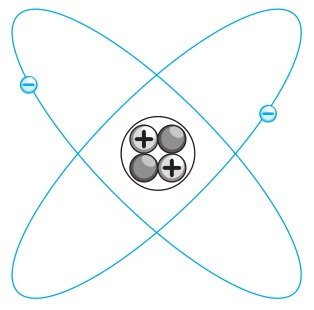
\includegraphics[scale=.8]{pics/Atom}
\caption{\textsc{Bohr}'sches Atommodell (Quelle: Hoffmann, Dirk)}
\label{Abb:Atom}
\end{center}
\end{figure}


Der \emph{Atomkern} besteht dabei aus Protonen (+) und Neutronen (elektrisch neutral).
Um den Kern kreisen die Elektronen (-) in der Atomhülle.
Die Atomhülle ist in mehrere Schalen unterteilt. Die $n$-te Schale kann dabei $2n^2$ Elektronen beherbergen.



In der Physik unterschiedet man zwischen Isolatoren, Halbleitern und Leitern.
Während Isolatoren nur sehr schlecht elektrischen Strom leiten, sind Leiter (wie das der Name schon sagt), sehr gute Stromleiter.
Halbleiter bilden eine Art Zwischenstadium.

Abbildung \ref{Abb:Energieniveau} zeigt den Unterschied in den Energieniveaus.


\begin{figure}[htp]
\begin{center}
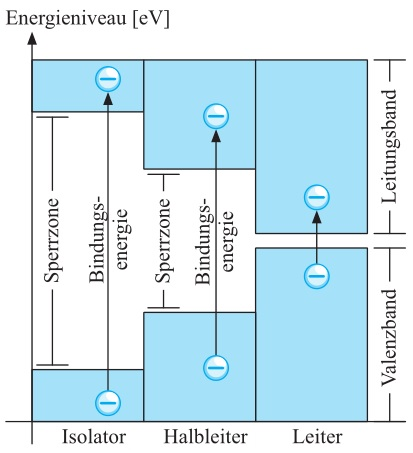
\includegraphics[scale=.8]{pics/Bindungsenergie}
\caption{Isolator, Halbleiter und Leiter mit ihren Energieniveaus (Quelle: Hoffmann, Dirk)}
\label{Abb:Energieniveau}
\end{center}
\end{figure}

Abgebildet ist dabei das Valenzband (unten).
Dies ist das Energieniveau, bei dem sich Elektronen als Valenzelektronen verhalten, d.h. dass sie sich auf der äußeren ungesättigten Schale eines Atoms befinden.

Darüber ist das Leitungsband abgebildet.
Dies ist das Energieniveau, bei dem sich Elektronen als freie Ladungsträger verhalten, d.h. dass sie sich frei im Atomverbund bewegen können, da sie sich durch Energieeinwirkung aus der Schale getrennt haben.
Diese freien Ladungsträger können den gerichteten Stromfluss bilden, der durch eine Spannungsquelle induziert wird.

Wie abgebildet ist, gibt es zwischen diesen Bändern eine Sperrzone.
Diese ist bei Isolatoren sehr groß.
Das bedeutet, man muss bei Isolatoren sehr viel Energie aufwenden, um ein Elektron vom Valenzband in das Leitungsband zu befördern, um freie Ladungsträger zu bekommen.

Die Sperrzone bei Leitern ist nur sehr gering, sodass man nur wenig Energie aufbringen muss, um freie Ladungsträger zu bekommen.

Halbleiter haben eine schmalere Sperrzone als Isolatoren.
Die Breite der Sperrzone kann in einigen Halbleitern beeinflusst werden.

Halbleiter sind als Kristalle angeordnet.
Zu solchen Kristallen ordnen sich beispielsweise Silizium und Germanium an, die deshalb typische Halbleiter sind (siehe Abbildung \ref{Abb:Kristall}).
Diese Anordnung geschieht, da diese Elemente vier Elektronen in ihrer äußersten Schale besitzen.
Damit diese Schale gesättigt wird (8 Elektronen), verbinden sich diese so, dass jedes der Elemente 8 Elektronen besitzt.


\begin{figure}[htp]
\begin{center}
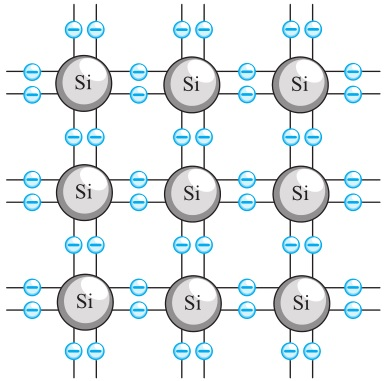
\includegraphics[scale=.8]{pics/Kristall}
\caption{Kristall aus Siliziumatomen (zweidim. Anordnung) (Quelle: Hoffmann, Dirk)}
\label{Abb:Kristall}
\end{center}
\end{figure}


Legt man an einen solchen Kristall eine Spannungsquelle an, bewegen sich freie Ladungsträger in diesem Kristall zum Pluspol (physikalische Stromrichtung).
Entsprechend entsteht ein Löcherstrom, der sich entgegen dieser Richtung zum Minuspol bewegt (technische Stromrichtung).
Dies ist in Abbildung \ref{Abb:Loecher}  dargestellt.

\begin{figure}[htp]
\begin{center}
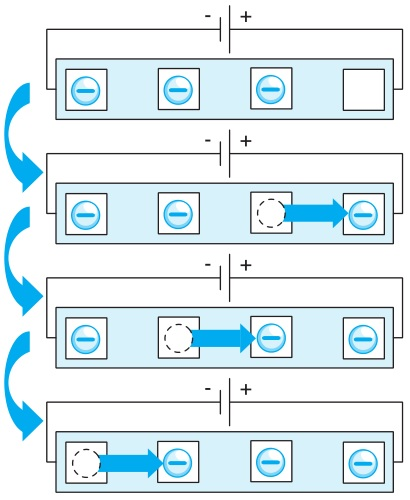
\includegraphics[scale=.7]{pics/Loecherstrom}
\caption{Kristall aus Siliziumatomen (zweidim. Anordnung) (Quelle: Hoffmann, Dirk)}
\label{Abb:Loecher}
\end{center}
\end{figure}

Diesen Löcherstrom beschreibt aber keine Bewegung von Elektronenlöchern (also freien Plätzen von Elektronen), sondern nur eine gedachte Bewegung.
Dies kann man sich vorstellen, wie in einem Kino.
Wenn in der Mitte ein Sitz frei bleibt, rückt ein Besucher nach, um besser sehen zu können.
Entsprechend kann sein Sitznachbar auch nachrücken, u.s.w.
Die Abbildung \ref{Abb:Kino} zeigt das Prinzip.
Dabei bewegst sich natürlich kein Kinositz, aber man könnte sagen, dass der freie Kinositz von rechts nach links durchwandert.
Ebenso verhällt es sich mit dem Löcherstrom.


\begin{figure}[htp]
\begin{center}
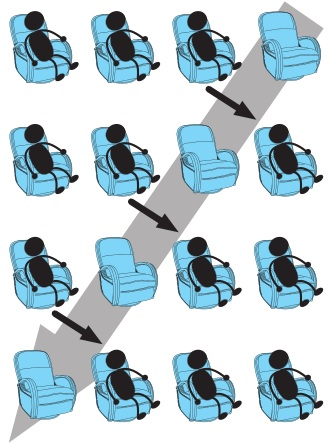
\includegraphics[scale=.7]{pics/Kino}
\caption{Der freie Kinositz bewegt sich gedacht nach links (Quelle: Hoffmann, Dirk)}
\label{Abb:Kino}
\end{center}
\end{figure}


Das Besetzen der Löcher (oder Defektelektronen) durch Elektronen nennt man \emph{Paarbildung}.
Durch eine angelegte Spannung wird es einem Elektron erleichtert seinen Platz frei zu geben, um ein benachbartes Elektronenloch zu besetzen.
Dabei lässt es (wie bei den Kinositzen) ein neues Elektronenloch zurück.

Diese Paarbildung wird durch eine erhöhte Energieeinwirkung erleichtert.
So kann man bei Halbleitern z.B. Wärme zuführen um diesen Effekt zu erleichtern.
Daraus ergibt sich, dass die Leitfähigkeit von Halbleitern durch Energieeinwirkung verbessert werden kann.



\section{Typische Halbleitersensoren}

%\begin{code}{1}
\begin{Aufgabe}
Implementiere in \textsc{Yenka} einen Gleichstromkreis, der aus einer Batterie, einer LED und (Electronic Components $\Rightarrow$ Inputs $\Rightarrow$ Sensors):
\begin{itemize}
\item[(a)] einem Thermistor (Heißleiter)
\item[(b)] einem LDR (with Lamp) (Fotowiderstand)
\end{itemize}
besteht.
Teste die Schaltungen und deren Funktionsweise.

\textbf{Hinweis:} Verringere den Eigenwiderstand des Heißleiters durch Doppelklick auf 1 $k\Omega$.
%\end{code}
\end{Aufgabe}

\begin{sich}
Ein \emph{Heißleiter} (NTC - Negative Temperature Coefficient) oder \emph{Thermistor} ist ein temperaturabhängiger Halbleitersensor.
Steigt die Umgebungstemperatur, so verringert sich der Widerstand des Halbleiters und die Leitfähigkeit und damit die Stromstärke steigt.
Anwendungen findet der Thermistor in Temperaturfühlern.

Ein \emph{Fotowiderstand} (LDR - Light Dependent Resistor) ist ein lichtabhängiger Halbleitersensor.
Steigt die einstrahlende Lichtintensität, so verringert sich der Widerstand des Halbleiters und die Leitfähigkeit und damit die Stromstärke steigt.
Anwendung findet der Fotowiderstand in Beleuchtungsstärkemessern und Flammenwächtern.
\end{sich}

Abbildung \ref{Abb:ntcldr} zeigt die beiden Schaltsymbole der Halbleitersensoren. Übernimm diese in dein Heft!

\begin{figure}[htp]
\begin{center}
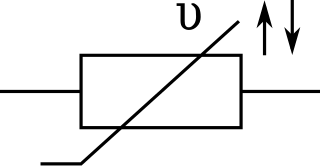
\includegraphics[scale=.4]{pics/ntc}
~~~~
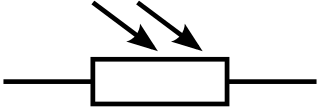
\includegraphics[scale=.5]{pics/ldr}
\caption{Schaltsymbol des NTC (links) und LDR (rechts) (Quelle: wikipedia.org)}
\label{Abb:ntcldr}
\end{center}
\end{figure}


%\begin{code}{1}
\begin{Aufgabe} \label{Aufg:SensorSimul}
Implementiere in \textsc{Yenka} einen Gleichstromkreis, der folgende Anwendungen simuliert:
\begin{itemize}
\item[(a)] Eine Alarmanlage, die anspringt, wenn die Temperatur im Raum über ca. 30 Grad Celsius springt. Als Alarm kann hierzu der Buzzer (Elcetronic Components $\Rightarrow$ Basic Components $\Rightarrow$ Symbolic) verwendet werden
\end{itemize}
\textbf{Hinweis:} Verringere den Eigenwiderstand des Halbleiterelements durch Doppelklick darauf!
\begin{itemize}
\item[(b)] Eine Solarzelle, die bei Lichteinstrahlung eine LED (ebenda) betreibt.
\item[\textcolor{red}{(ZA)}] \textcolor{red}{Eine Alarmanlage, die anspringt, wenn die Tür geöffnet wird. Die Tür ist durch einen Lichtsensor mit dem Buzzer gekoppelt, fällt kein Licht auf den Sensor, geht der Buzzer an. Verwende ein Relais (Inputs $\Rightarrow$ Switches)!}
\end{itemize}
\end{Aufgabe}
%\end{code}






\section{Die Halbleiterdiode}

%\begin{code}{1}
\begin{Aufgabe} \label{Aufg:DiodeTest}
Implementiere in Yenka einen Stromkreis bestehend aus einer Batterie, einer Diode (Electronic Components $\Rightarrow$ Analogue Processing $\Rightarrow$ Discrete Semiconductors) und einem Amperemeter (Lab Equipment $\Rightarrow$ Measurement).


\begin{itemize}
\item[(a)] Lege eine Tabelle für $U$ und $I$ an und miss die  Stromstärke $I$ für folgende Spannungen! Skizziere die Werte als Graph!

\begin{center}
\begin{tabular}{|c|c|c|c|c|c|c|c|c|c|}
\hline
$U$ in V & 0,1 & 0,2 & 0,3 & 0,4 & 0,5 & 0,6 & 0,7 & 0,8 & 0,9  \\ \hline
$I$ &&&&&&&&& \\ \hline
\end{tabular}
\end{center}

\item[(b)] Drehe die Diode um, sodass der Strom in die entgegengesetzte Richtung fließt!
Wiederhole die Messung für die folgenden Spannungen!

\begin{center}
\begin{tabular}{|c|c|c|c|c|c|c|}
\hline
$U$ in V & 0,5 & 1 & 10 & 25 & 50 & 51  \\ \hline
$I$ &&&&&& \\ \hline
\end{tabular}
\end{center}

\item[(c)] Formuliere für (a) und (b) eine Beobachtung, wie eine Halbleiterdiode arbeitet.

\item[\textcolor{red}{(ZA)}] \textcolor{red}{Wie ändert sich die Funktionsweise in (a) und (b) wenn man die Diode durch eine LED ersetzt?}

\end{itemize}
\end{Aufgabe}
%\end{code}



\begin{sich}
Eine Diode besitzt eine Durchlass- und eine Sperrrichtung.
In Durchlassrichtung fließt je mehr Strom, desto mehr Spannung anliegt.
Ab einem gewissen Schwellenwert (ca. 0,5 $V$) steigt der Stromfluss sehr stark an.

In Sperrrichtung lässt die Diode keinen Stromfluss zu.
Eine Diode kann deshalb als Sicherung in einem Stromkreis eingebaut werden, damit die Spannungsquelle nicht falschherum angeschlossen wird.

Eine Diode ist also wie eine Einbahnstraße, in die eine Richtung darf Strom fließen, in die andere nicht.
\end{sich}

Abbildung \ref{Abb:DiodeGraph} zeigt den Stromfluss einer Diode in Abhängigkeit der angelegten Spannung.
Dabei steht eine positive Spannung für das anlegen in Durchlassrichtung.
Ab ca. 0,5 $V$ (Schwellspannung) steigt der Stromfluss stark an.

Negative Spannungen geben die Polung in Sperrrichtung an.
Hier fließt kein oder nur sehr wenig Strom (Sperrbereich).
Ist der Durchbruchbereich erreicht, wird die Diode zerstört.


\begin{figure}[ht]
\begin{center}
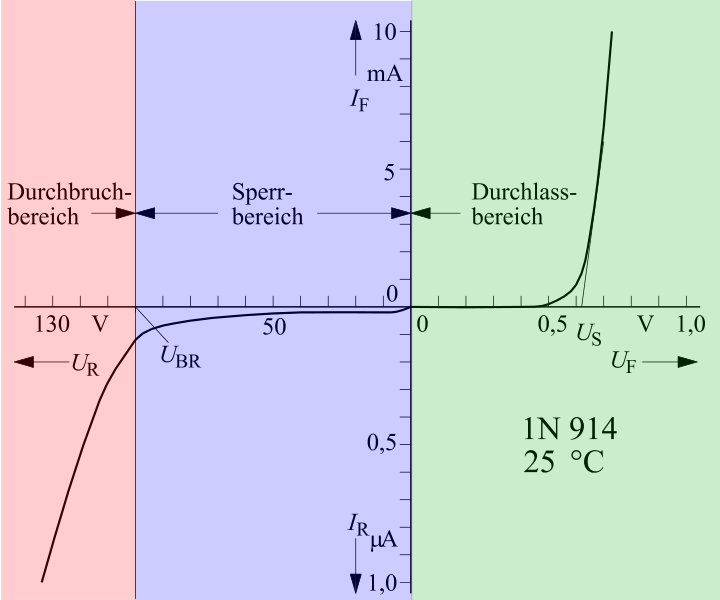
\includegraphics[scale=.6]{pics/diodegraph}
\caption{Stromfluss einer Diode abhängig von der angelegten Spannung (Quelle: wikimedia.org)}
\label{Abb:DiodeGraph}
\end{center}
\end{figure}


%\begin{code}{1}
\begin{Zusatzaufgabe}
Recherchiere im Internet zu den folgenden Fragen:
\begin{itemize}
\item Was bezeichnet das Dotieren eines Halbleiters und welche Formen gibt es?
\item Durch welche Dotierungen wird eine Diode gebildet und wie verhalten sich die Dotierungen wenn keine Spannung, Spannung in Sperrrichtung und Spannung in Durchlassrichtung angelegt wird?
\item Was bezeichnet die \emph{Schwellspannung}?
\item Was ist eine LED genau und wie ist diese mit der Diode "'verwandt"'?
\end{itemize}
\end{Zusatzaufgabe}
%\end{code}


\begin{sich}
Die folgende Abbildung zeigt, in welcher Richtung das Schaltzeichen einer Diode an den Pluspol angelegt werden muss, damit sie durchlässig (links) ist, oder sperrt (rechts).
%\begin{figure}
\begin{center}
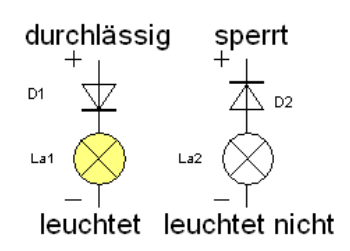
\includegraphics[scale=.7]{pics/diodenrichtung}
%\caption{Durchlass- und Sperrrichtung einer Diode (Quelle: strippenstrolch.de)}
%\label{Abb:Diodenrichtung}

\small{Quelle: strippenstrolch.de}
\end{center}
%\end{figure}
\end{sich}



%\begin{code}{1}
\begin{Aufgabe} \label{Aufg:Diodenlogik}
%\parpic[r][t]{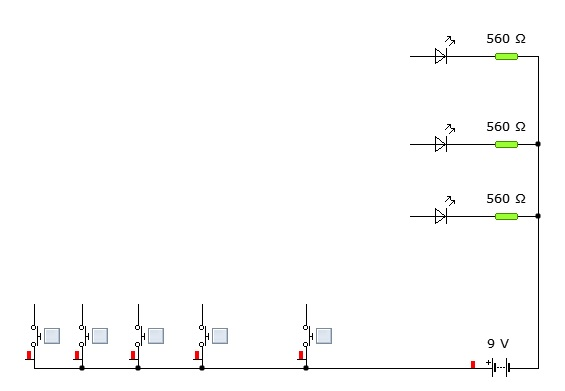
\includegraphics[scale=.4]{pics/diodenlogik}}

In der untenstehenden Abbildung sind die Schalter 1 bis 5 (von links nach rechts), sowie eine rote, eine gelbe und eine grüne LED (von oben nach unten) gegeben.
Vervollständige die Schaltung durch Verbindungen und Dioden, sodass

\begin{center}
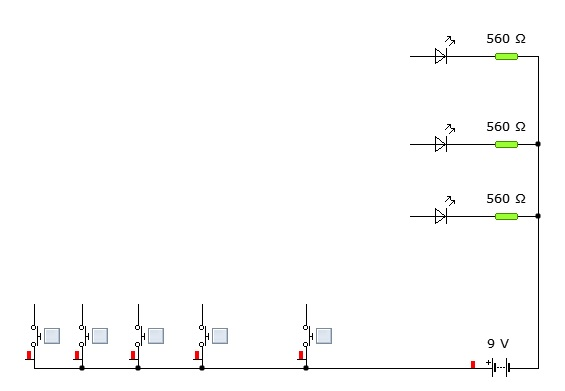
\includegraphics[scale=.9]{pics/diodenlogik}
\end{center}

\begin{itemize}
\item die rote LED beim Drücken von Schalter 1 leuchtet,
\item die gelbe LED beim Drücken von Schalter 2 leuchtet,
\item die grüne LED beim Drücken von Schalter 3 leuchtet sowie
\item die rote und gelbe LED beim Drücken von Schalter 4 leuchten und
\item alle LEDs beim Drücken von Schalter 5 leuchten.
\end{itemize}
\end{Aufgabe}
%\end{code}








%\newpage
%\setcounter{subsection}{2}
\section{Der Bipolartransistor}


Ein Bipolartransistor besteht aus folgenden drei Anschlüssen, die in Abbildung \ref{Abb:Bipolartransistor} dargestellt sind.


\begin{figure}[h]
\begin{sich}
\begin{center}
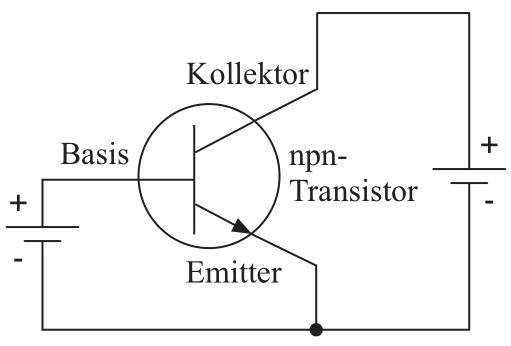
\includegraphics[scale=.4]{pics/transistorbegriffe}
\caption{Begriffe am Transistor (Quelle: D. Hoffmann)}
\label{Abb:Bipolartransistor}
\end{center}
\end{sich}
\end{figure}


%\begin{code}{1}
\begin{Aufgabe}
Implementiere in \textsc{Yenka} die untenstehende Schaltung (Electronic Components $\Rightarrow$ Analogue Processing $\Rightarrow$ Discrete Semiconductors $\Rightarrow$ NPN Transistor).
Bestimme das Verhältnis der Stromstärke am Kollektor $I_C$ zu der Stromstärke an der Basis $I_B$ für die folgenden Widerstandswerte:
\begin{align*}
R=4~k\Omega, 8~k\Omega, 15~k\Omega, 25 ~k\Omega, 50 ~k\Omega
\end{align*}
Formuliere eine Vermutung über die Funktionsweise eines Transistors!
\begin{itemize}
\item[(ZA)] Welcher funktionelle Zusammenhang besteht zwischen den Stromflüssen? Wie würde ein entsprechender Graph charakteristisch aussehen?
\end{itemize}

%\begin{figure}[h]
\begin{center}
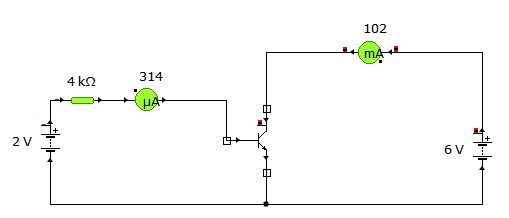
\includegraphics[scale=.8]{pics/transistor.jpg}
\end{center}
%\caption{Aufbau aus Arbeits- und Steuerstromkreis}
%\end{figure}
\end{Aufgabe}
%\end{code}


%\newpage
\begin{sich}
Das Verhältnis der Kollektor- zur Basisstromstärke wird auch Stromverstär\-kungsfaktor eines Transistors genannt.

\begin{align*}
\beta = \frac{I_C}{I_B}
\end{align*}

Ein kleiner Basisstrom (Steuerstromkreis) bewirkt einen großen Kollektorstrom (im Arbeitsstromkreis), wie in Abbildung \ref{Abb:Verst} dargestellt. Ein Transistor wird deshalb als elektronische Ansteuerung verwendet.

%\begin{figure}[htp] 
\begin{center}
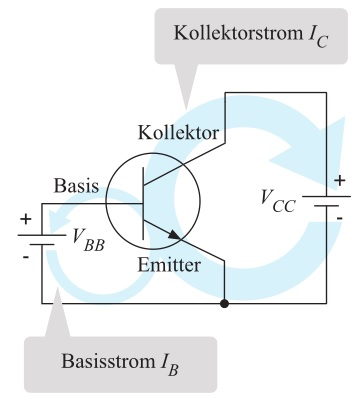
\includegraphics[scale=.6]{pics/StromTrans}
\end{center}
%\caption{Verstärkerwirkung eines Transistors.}
\label{Abb:Verst}
%\end{figure}
\end{sich}


%\newpage
\begin{ZW}
Ein npn-Bipolartransistor besteht aus zwei n- und einem p-dotierten Halbleiter, die wie in der Abbildung zusammengesetzt werden:

%\begin{figure}[h]
\begin{center}
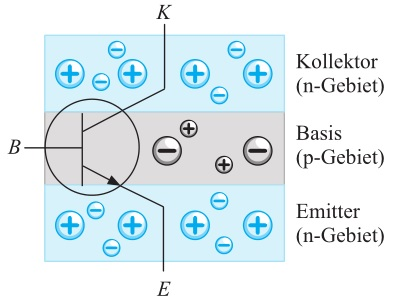
\includegraphics[scale=.8]{pics/AufbauTrans}
\end{center}
%\caption{Aufbau aus dotierten Halbleitern.}
%\end{figure}

Im Folgenden soll geklärt werden, warum ein nur kleiner Strom an der Basis-Emitter-Strecke (Steuerstromkreis) einen großen Strom an der Kollektor-Emitter-Strecke (Arbeitsstromkreis) hervorruft.
Diese Eigenschaft, die von $\beta$ abhängt, nennt man die Verstärkerwirkung eines Transistors (siehe Abbildung \ref{Abb:Verst}).




\begin{Aufgabe} \label{Aufg:npn}
Zur Vorüberlegung und zum besseren Verständnis, mache dir zunächst Gedanken, wie die n- bzw- p-Schicht bei angelegter Spannung agiert, wenn eine Spannung an der Kollektor-Emitter-Strecke ($U_{CE}$) anliegt und ...

\begin{itemize}
\item[(a)] keine Spannung an der Basis-Emitter-Strecke anliegt ($I_B=0$)
\item[(b)] eine Spannung an der Basis-Emitter-Strecke anliegt ($I_B>0$)
\end{itemize}
\end{Aufgabe}


\begin{Loesung}[zu Aufgabe \ref{Aufg:npn}]

Siehe dazu Abbildung \ref{Abb:TransSperr}.


%\begin{figure}[h] 
\begin{center}
\begin{tabular}{ccc}
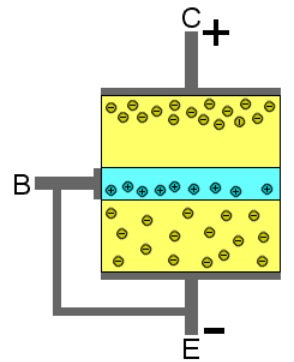
\includegraphics[scale=.6]{pics/gespTrans}
& ~~~~ &
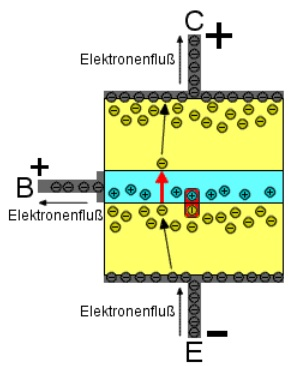
\includegraphics[scale=.6]{pics/durchTrans} \\
(a) && (b)
\end{tabular}
\end{center}
%\caption{(a) Der Transistor sperrt, die Raumladungszone zwischen der oberen np-Schicht vergrößert sich; (b) Der Transistor lässt Stromfluss durch.}
\label{Abb:TransSperr}
%\end{figure}

\end{Loesung}
%\end{ZW}
%
%%\newpage
%\begin{ZW}
\begin{itemize}
\item[(a)] Ist die Spannung der Basis-Emitter-Strecke gleich 0, fließt folglich auch kein Basisstrom. Damit ist der pn-Übergang der Kollektor-Emitter-Strecke in Sperrrichtung betrieben, da die n-Schicht des Kollektors am Pluspol angeschlossen ist und die p-Schicht der Basis über den Emitter am Minuspol angeschlossen ist. Somit sperrt der Transistor und es fließt auch kein Strom auf der Kollektor-Emitter-Strecke. Prinzipiell ist der Widerstand des Transistors damit unendlich groß. 
\item[(b)] Ist hingegen eine Spannung an der Basis-Emitter-Strecke angeschlossen wird der np-Übergang an der Basis-Emitter-Strecke in Durchlassrichtung betrieben. Wie in einer Diode rekombinieren die freien Ladungsträger in der Grenzschicht zwischen p- und n-Gebiet miteinander. Ab einer gewissen Schwellspannung kann der Strom ungehindert über die Basis-Emitter-Strecke fließen.

Durch die Rekombination gehen die Elektronen der Emitter-Schicht daher in die p-Schicht über. Da die Basis nur eine sehr dünne p-Schicht besitzt und der Emitter aber mit einer starken Dotierung bestückt ist, verschwindet durch die Rekombination die p-Schicht und wird zunächst neutral. Da immer mehr Elektronen nachkommen, können diese nun ungehindert in die n-Schicht des Kollektors, durch den Sog der Kollektor-Spannung, gelangen und es entsteht ein großer Kollektor-Emitter-Strom.
\end{itemize}

Die Computer der ersten Generation wurden zunächst aus Relais gebaut. Diese elektronisch steuerbaren Schalter waren jedoch groß, laut und vor allem langsam.
Die Computer waren demnach raumgroß und an einen Rechner als \emph{Personal Computer} war dabei noch nicht zu denken, denn nur Universitäten, Regierungseinrichtungen und das Militär konnten sich ein solch teures und großes Gerät leisten.
In der zweiten Generation verwendete man hingegen Radioröhren als Schalter. Diese waren bereits wesentlich schneller, jedoch nicht kleiner.

Die dritte und vierte Generation unterscheiden sich in der Art der Konstruktion. Computer der vierten Generation, wie man sie seit den 1980er-Jahren kennt, besitzen \emph{integrierte Schaltkreise}.
\end{ZW}

In der Computertechnik wird der Transistor jedoch eher als elektronisch steuerbarer Schalter verwendet. Der Transistor als Schalter wird bereits seit der dritten Computergeneration verbaut, dabei handelt es sich aber um Feldeffekttransistoren, deren physikalische Erklärung jedoch etwas zu schwierig für uns ist.
Im Folgenden wird auf den Einsatz des Transistors als Schaltelement eingegangen. 



%\begin{code}{1}
\begin{Aufgabe}
\hfill \par
\vspace*{-.7cm}
%\begin{figure}[htp] 
\begin{center}
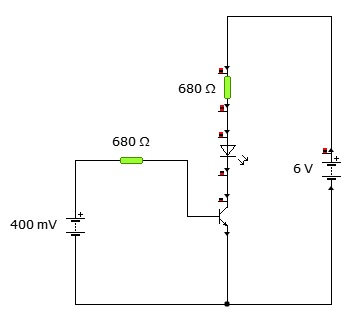
\includegraphics[scale=.9]{pics/eschalter}
\captionof{figure}{Transistor als Schalter.}
\label{Abb:eschalter}
\end{center}
%\end{figure}

Implementiere die Schaltung aus Abbildung \ref{Abb:eschalter} 
in \textsc{Yenka}!
Beobachte den Zustand der LED für die beiden Werte $U_{BE}=0,4 ~V$ und $U_{BE}=5~V$ und beantworte die untenstehenden Fragen!
%\vspace{1.7cm}
\begin{itemize}
\item[(a)] Wie ist der Zustand der LED mit Hilfe der Funktionsweise des Transistors zu erklären?
\item[(b)] Diese Schaltung wird als elektronischer Schalter bezeichnet. Welche Verwandtschaft besteht zu einem mechanischem Schalter?
\end{itemize}
\end{Aufgabe}
%\end{code}

Zum Schalten lassen wir nur zwei verschiedene Spannungswerte für $U_{BE}$ zu.
Der erste wird als 0 oder $L$ bezeichnet und bedeutet \emph{niedrige Spannung}. Der zweite wird als 1 oder $H$ bezeichnet und bedeutet \emph{hohe Spannung}.

Die LED in Abbildung \ref{Abb:eschalter} ist nur als Repräsentant anzusehen. Ersetzt man diese durch einen Spannungsmesser und ließt die Spannung $U_A$ daran ab, ergeben sich für 0 und 1 die folgenden Spannungsbereiche:

\begin{sich}
\hfill \par
\vspace*{-.7cm}
\begin{itemize}
\item für $U_{BE} < 0,8V$ gilt logisch 0
\item für $U_{BE} > 2,0V$ gilt logisch 1
\item für $U_{A} < 0,4V$ gilt logisch 0
\item für $U_{A} > 2,4V$ gilt logisch 1
\item dazwischen liegt der "'verbotener Bereich"', da nicht sicher ist, ob dies 0 oder 1 entspricht.
\end{itemize}
\end{sich}



Der Transistor kann ebenso als Inverter verbaut werden. Das bedeutet, dass für 0 am Eingang 1 am Ausgang anliegt und umgekehrt.


%\begin{code}{1}
\begin{Aufgabe} \label{Aufg:Inverter}
Implementiere in \textsc{Yenka} eine Schaltung aus einem npn-Transistor und einer LED, die ein Eingabesignal invertiert.
D.h. wenn $U_{BE}$ logisch 0 ist, soll die LED leuchten (log. 1), wenn $U_{BE}$ logisch 1 ist, soll die LED nicht leuchten (log. 0)!

%\end{code}

\textbf{Hilfestellung:} Wenn du nicht voran kommst, markiere den folgenden Text und füge ihn in ein Textverarbeitungsprogramm ein um eine Hilfestellung zu bekommen: 
\textcolor{grau}{Die Schaltung ist ähnlich zu der des elektronischen Schalters. Die LED muss lediglich umpositioniert werden, sodass sie nicht leuchtet, wenn der Transistor einen kleinen Widerstand hat und umgekehrt.}
\end{Aufgabe}

%\begin{code}{1}
\begin{Aufgabe} \label{Aufg:Daemmerung}
Benutze die Eigenschaft des Inverters und implementiere eine Schaltung in \textsc{Yenka} für folgendes Problem:

\begin{quote}
Bei einer Dämmerungsschaltung für Straßenlaternen leuchtet eine Reihe von Lampen, wenn die Umgebungshelligkeit unter einen kritischen Wert sinkt. Ist es hell genug, bleiben die Lampen ausgeschaltet.
\end{quote}

\begin{itemize}
\item[(ZA)] Stelle den Arbeitspunkt so ein, dass die LEDs nicht erst bei vollkommener Dunkelheit, sondern auch bereits bei Dämmerlicht anspringen.
\end{itemize}

\end{Aufgabe}
%\end{code}


%\begin{code}{1}
\begin{Aufgabe} \label{Aufg:TransistorKomplex}
Öffne im Tauschordner die Datei Alarmanlage.yka.
Implementiere mit den bisher verwendeten Halbleiterbauelementen eine Alarmanlage (als Arbeitsstromkreis), die folgende Anforderungen genügt (bis (N2) solltest du es schaffen):
\begin{itemize}
\item[\textcolor{green}{(N1)}] Ein Lichtsensor wird an der Tür angebracht. Dieser besteht aus einem Laser (dargestellt durch eine Lampe) und trifft auf einen Fotowiderstand. Wird der Laser unterbrochen (Schalter offen) fließt ein Basisstrom und ein Buzzer springt an! Trifft der Laser ungehindert auf den Fotowiderstand (Schalter geschlossen), fließt kein Basisstrom und der Buzzer bleibt stumm.
Der Alarm soll von dem Buzzer ausgelöst werden.

Hinweis: \textcolor{grau}{Überlege dir, was Eingang und was Ausgang darstellt und wie du die Eigenschaft des Ausgangs invertieren kannst.}
\item[\textcolor{blue}{(N2)}] Zusätzlich soll die Alarmanlage auch anspringen, wenn die Zimmertemperatur mehr als ca. 30 Grad beträgt.

Hiweis \textcolor{grau}{Überlege dir, was invertiert werden soll und was nicht. Die Richtung des Stromflusses ist in dieser Aufgabe auch sehr wichtig!}
\item[\textcolor{red}{(N3)}] Zusätzlich soll die Alarmanlage einen Rauchmelder besitzen. Dieser soll durch einen Lichtsensor realisiert werden, der zudem Alarm auslöst, wenn die Umgebungshelligkeit zu gering wird. Achte darauf, dass der Alarm nicht erst angeht, wenn vollkommene Dunkelheit herrscht.
\end{itemize}
\end{Aufgabe}
%\end{code}



\section[Der Schwellenwertschalter (Zusatzwissen)]{Der Schwellenwertschalter}
\begin{ZW}
Ein weiteres Halbleiterbauelement, dass in Schaltungen viel zum Einsatz kommt ist der Schwellenwertschalter, im Besonderen der \emph{Schmitt-Trigger}.

\begin{Aufgabe} \label{Aufg:SchmittTest}
Öffne im Tauschordner die Datei \emph{Schmitt-Inverter.yka}!
\begin{itemize}
\item[(a)] Fülle die Tabelle aus!
\item[(b)] Formuliere die Arbeitsweise des Bauelements!
\item[(c)] Skizziere einen Graphen, wobei an der $x$-Achse die Eingangsspannung und an der $y$-Achse $U_2$ abgetragen ist!
\item[(ZA)] Welchen Vorteil könnte das unterschiedliche Schaltverhalten beim Auf- und Absteigen besitzen?
\end{itemize}
\end{Aufgabe}



\textsc{Yenka} bietet uns leider nur den sogenannten \emph{Schmitt-Inverter}, dieser funktioniert wie ein \emph{Schmitt-Trigger}, invertiert das Signal aber noch zusätzlich.

Der \emph{Schmitt-Inverter} lässt daher die anliegende Spannung ab einem gewissen Pegelwert durch, invertiert dann aber noch das Verhalten. Das heißt, unter der Pegelspannung $U_P$ ist der Ausgang auf log. 1; über der Pegelspannung $U_P$ ist der Ausgang auf log. 0.

\par \hfill \par

Beim Hoch- und Runterdrehen der Spannung fällt auf, dass die Pegelspannung nicht die gleiche für beide Prozesse ist.
Das bedeutet, dass beim Hochregeln später die Pegelspannung erreicht wird (ab ca. $3V$) als beim Runterregeln (ab ca. $2V$). Diese Eigenschaft wird \emph{Hysterese} genannt und ist dafür da, dass kleine Spannungsschwankungen um den Schwellwert noch keine Auswirkungen auf die Ausgangsspannung haben.

Das Bauelement wird unter Anderem als Korrektur in Kabeln über weite Entfernungen verwendet, weil das Signal langsam abgeschwächt wird. Darüber hinaus kann es auch dazu verwendet werden, aus einem analogen Eingang (wie Lichtintensität) einen Wert als niedrig (0) oder hoch (1) darzustellen.


\begin{Aufgabe}
Öffne im Tauschordner die Schaltung \emph{Aufbau Schmitt Inverter.yka}
\begin{itemize}
\item[(a)] Teste die Schaltung für verschiedene Eingangsspannungen und beobachte das Verhalten der LED!
\item[(b)] Überlege dir Antworten zu den folgenden Fragen:
\begin{itemize}
\item Warum leuchtet die LED bei geringer Eingangsspannung?
\item Warum leuchtet die LED nicht bei hoher Eingangsspannung?
\end{itemize}
\end{itemize}
\end{Aufgabe}


\begin{Aufgabe}
Öffne im Tauschordner \emph{Dämmerungsschaltung.yka}!
\begin{itemize}
\item[(a)] Verändere die Schaltung so, dass ein Schmitt-Inverter den Transistor ansteuert! (Denke daran, dass der Schmitt-Inverter bereits das Signal negiert)
\item[(b)] Was ist der Vorteil des Schwellenwertschalters in dieser Schaltung?
\end{itemize}
\textbf{Hinweis:} \textcolor{red}{Benutze einen Widerstand als Spannungsteiler für den LDR!}
\end{Aufgabe}
\end{ZW}


\section*{Zusammenfassung}

\begin{center}
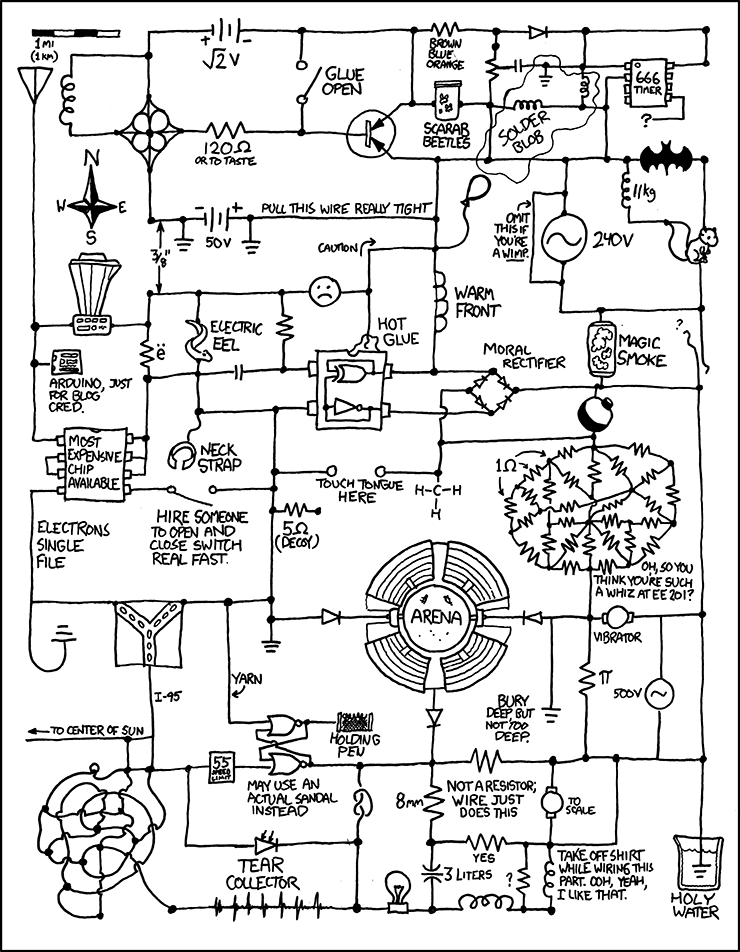
\includegraphics[scale=.55]{com/circuit}
\\
Quelle: xkcd.com
\end{center}

In der Computer- und Informationstechnik sind Halbleiter unabdingbar.
Ihren chemischen und physikalischen Eigenschaften haben wir zu verdanken, dass Prozessoren und Chips mit der Leistung und Integrationsdichte (Transistoren pro Fläche) wie wir sie heute kennen, überhaupt möglich sind.
Der Transistor kommt als Schaltelement in jedem heutigen Computerchip vor und ist dabei mehrere tausendmal schneller als die früher benutzten Röhrentrioden.
Dabei setzt man aber auf Feldeffekttranistoren, statt auf Bipolartransistoren, deren Funktionsweise jedoch dieselbe ist.

Im nächsten Abschnitt wird weiter darauf eingegangen, wie aus einem Transistor ein Logikgatter entsteht.